\documentclass[12pt,a4paper]{article}

% ===== Packages =====
\usepackage[utf8]{inputenc}
\usepackage[T1]{fontenc}
\usepackage{amsmath,amssymb,amsfonts,amsthm}
\usepackage[margin=2.5cm]{geometry}
\usepackage{hyperref}
\usepackage{xcolor}
\usepackage{booktabs}
\usepackage{graphicx}
\usepackage{float}
\usepackage{enumitem}
\usepackage{mathtools}
\usepackage{cite}

\hypersetup{
  colorlinks=true,
  linkcolor=blue!60!black,
  citecolor=green!50!black,
  urlcolor=blue!70!black,
  pdfauthor={David Alfyorov, Igor Shnyukov},
  pdftitle={Universal absence of the scalar graviton in spectral causal theory},
}

\newtheorem{theorem}{Theorem}
\newtheorem{lemma}[theorem]{Lemma}
\newtheorem{corollary}[theorem]{Corollary}
\newtheorem{proposition}[theorem]{Proposition}
\newtheorem{remark}[theorem]{Remark}

\newcommand{\Lam}{\Lambda}
\newcommand{\Tr}{\operatorname{Tr}}
\newcommand{\PiTT}{\Pi_{\mathrm{TT}}}
\newcommand{\Pis}{\Pi_{s}}
\newcommand{\alphaR}{\alpha_R}
\newcommand{\alphaC}{\alpha_C}
\newcommand{\half}{\tfrac{1}{2}}
\newcommand{\dd}{\mathrm{d}}
\newcommand{\ee}{\mathrm{e}}

\title{\textbf{Absence of a real scalar graviton pole\\
in spectral causal theory}}
\author{David Alfyorov, Igor Shnyukov}
\date{April 2026}

\begin{document}
\maketitle

\begin{abstract}
We prove that spectral causal theory (SCT), a one-loop effective theory of
gravity derived from the spectral action principle with Standard Model matter
content, propagates exactly two gravitational degrees of freedom, the same as
general relativity. The scalar propagator denominator satisfies $\Pis(z,\xi) > 1$
for all Euclidean momenta $z > 0$ and all values of the Higgs
non-minimal coupling $\xi$, including conformal coupling $\xi = 1/6$:
no real scalar mass pole exists.
The mechanism is the conformal invariance of spin-$\half$ and spin-$1$ fields
in $d = 4$: their positive contributions to the $R^2$ form factor dominate
the scalar sector at all scales.
The spin-2 mode is quantized as an Anselmi--Piva fakeon, contributing zero
asymptotic degrees of freedom.  (The fakeon prescription is formulated for
propagators with finitely many poles; its extension to the full
entire-function propagator, which has infinitely many complex zeros,
requires a convergence proof not provided here.)
We derive the nonlocal spin-2 mass $m_2 = 1.554\,\Lam$ from the unique
positive zero of $\PiTT$, show that no additional \emph{real} massive modes
exist, compute a dedicated torsion-balance bound ($\Lam > 3.53$~meV),
and characterize the robustness of the no-scalaron theorem under
extensions of the matter sector.
The Standard Model lies deep within the safe region: $4.7\times$ above the
critical fermion ratio and $12\times$ above the critical vector ratio.
\end{abstract}

\tableofcontents

% ======================================================================
\section{Introduction}
\label{sec:intro}
% ======================================================================

The one-loop gravitational effective action for quantum fields on curved
backgrounds takes the universal form~\cite{BV1985,CZ2012}
\begin{equation}\label{eq:action}
  \Gamma^{(1)} = \frac{1}{16\pi^2}
  \int \dd^4x\,\sqrt{g}\;\bigl[
    \alphaC(\Box/\Lam^2)\,C_{\mu\nu\rho\sigma}C^{\mu\nu\rho\sigma}
    + \alphaR(\Box/\Lam^2,\xi)\,R^2
  \bigr],
\end{equation}
where $\alphaC$ and $\alphaR$ are nonlocal form factors generated by
the master function $\varphi(x) = \int_0^1 \dd\alpha\;\ee^{-x\alpha(1-\alpha)}$,
$\Lam$ is the spectral cutoff scale, and $\xi$ is the Higgs non-minimal
coupling.

In spectral causal theory (SCT), the action~\eqref{eq:action} is
\emph{derived} from the spectral action principle $S = \Tr\,f(D^2/\Lam^2)$
applied to the spectral triple of the Standard Model~\cite{CC1996,CCM2007},
with all coefficients fixed by the SM field content. The spin-2 massive
mode ($\PiTT$ zero) is quantized using the Anselmi--Piva fakeon
prescription~\cite{Anselmi2017,AP2018}, which projects it out of the
physical spectrum and ensures perturbative unitarity.

A central question for any higher-derivative gravity theory is:
\emph{how many propagating degrees of freedom does it have?}
Stelle gravity~\cite{Stelle1977} has eight (including a massive scalar
and a massive spin-2 ghost). $f(R)$ theories~\cite{Sotiriou2010} have
three (the massless graviton plus a scalaron).
Infinite-derivative gravity (IDG)~\cite{BMS2012} eliminates ghosts by
postulating an entire-function form factor, but the particle spectrum
depends on a free function.

In this paper, we prove that SCT has exactly \emph{two} propagating
degrees of freedom (the same as GR) under no additional assumptions
beyond the SM spectrum and the fakeon prescription. The scalar gravitational
mode is universally absent: $\Pis(z,\xi) > 1$ for all $z > 0$ and all $\xi$.
This is a parameter-free prediction.


% ======================================================================
\section{Propagator structure}
\label{sec:propagator}
% ======================================================================

The linearized SCT propagator on flat background decomposes via
Barnes--Rivers projectors into spin-2 (transverse-traceless, TT) and
spin-0 (scalar) sectors~\cite{Alfyorov2025a}:
\begin{equation}\label{eq:propagator}
  G^{-1}_{\mu\nu\rho\sigma}(k)
  = k^2\;\bigl[
    \PiTT(z)\,P^{(2)}_{\mu\nu\rho\sigma}
    + \Pis(z,\xi)\,P^{(0\text{-}s)}_{\mu\nu\rho\sigma}
  \bigr],
\end{equation}
where $z = k^2/\Lam^2$ and the denominator functions are
\begin{align}
  \PiTT(z) &= 1 + \frac{13}{60}\,z\,\hat{F}_1(z), \label{eq:PiTT} \\
  \Pis(z,\xi) &= 1 + 6\Bigl(\xi - \frac{1}{6}\Bigr)^{\!2}\;z\;\hat{F}_2(z,\xi).
    \label{eq:Pis}
\end{align}
Here $\hat{F}_{1,2}$ are normalized shape functions ($\hat{F}(0) = 1$)
of the Weyl and Ricci form factors, and the numerical coefficients
$\alphaC = 13/120$ and $\alphaR(\xi) = 2(\xi-1/6)^2$ are determined
by the SM spectrum ($N_s = 4$ real scalars, $N_f = 45$ Weyl fermions,
$N_v = 12$ gauge bosons)~\cite{Alfyorov2025a}.


\subsection{Spin-2 sector}

\begin{figure}[t]
\centering
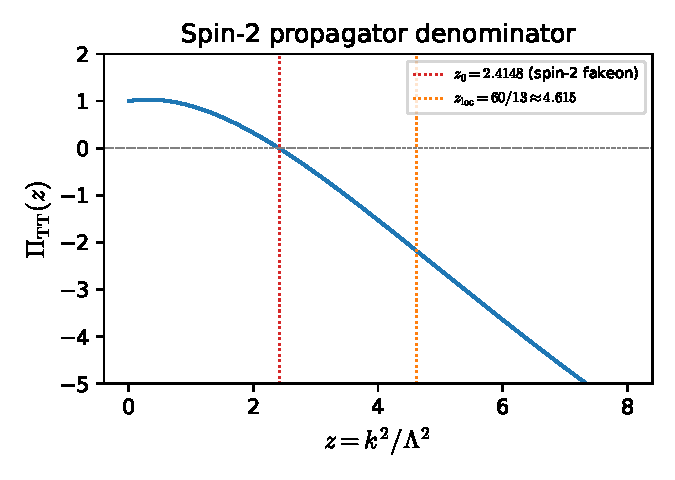
\includegraphics[width=0.85\columnwidth]{figures/fig4_pi_tt.pdf}
\caption{The spin-2 propagator denominator $\PiTT(z)$ on the real axis.
The unique positive zero at $z_0 = 2.4149$ (red dashed) defines the
spin-2 fakeon mass $m_2 = \Lam\sqrt{z_0} = 1.554\,\Lam$.
The local approximation zero $z_{\mathrm{loc}} = 60/13$ (orange dashed)
overestimates the exact value by 38\%.}
\label{fig:pi-tt}
\end{figure}

$\PiTT$ has exactly one positive real zero at $z_0 \in (2, 5/2)$,
with $z_0 = 2.4149$ (30-digit precision). The proof of uniqueness
proceeds by showing $\PiTT(z) > 0$ on $(0, 2]$ (via a concave
polynomial lower bound), $\PiTT(5/2) < 0$ (via an upper bound),
and $\PiTT'(z_*) < 0$ at any positive zero $z_*$ (via the
recurrence~\eqref{eq:recurrence}), which precludes a return to zero
by contradiction. The zero corresponds to the massive spin-2 mode
with mass
\begin{equation}\label{eq:m2}
  m_2 = \Lam\sqrt{z_0} = 1.554\,\Lam.
\end{equation}
In the local (small-$z$) approximation, $z_0^{\mathrm{loc}} = 60/13$
gives $m_2^{\mathrm{loc}} = 2.148\,\Lam$, which overestimates the
exact value by 38\%.
The spin-2 mode is quantized as a fakeon~\cite{Anselmi2017}:
it contributes zero asymptotic degrees of freedom and produces
a single-Yukawa correction to the static potential (the scalar
Yukawa is absent by Theorem~\ref{thm:no-scalaron}).


\subsection{Scalar sector: reformulation}

Using $\alphaR(0,\xi) = 2(\xi - 1/6)^2$ and the definition
$\hat{F}_2 = \alphaR(z,\xi)/\alphaR(0,\xi)$, the product
\begin{equation}\label{eq:product}
  6\Bigl(\xi - \frac{1}{6}\Bigr)^{\!2}\;\hat{F}_2(z,\xi)
  = 3\,\alphaR(z,\xi),
\end{equation}
where $\alphaR(z,\xi)$ is the full $z$-dependent total $R^2$ form factor:
\begin{equation}\label{eq:alphaR}
  \alphaR(z,\xi) = N_s\,h_R^{(0)}(z,\xi)
    + \frac{N_f}{2}\,h_R^{(1/2)}(z)
    + N_v\,h_R^{(1)}(z).
\end{equation}
Using~\eqref{eq:product}, the scalar propagator denominator takes
the universal form
\begin{equation}\label{eq:Pis-reformulated}
  \boxed{\Pis(z,\xi) = 1 + 3\,z\,\alphaR(z,\xi),}
\end{equation}
valid for all $\xi$ including $\xi = 1/6$. (At $\xi = 1/6$ the
factorized form~\eqref{eq:Pis} involves a $0/0$ indeterminacy in
$\hat{F}_2$; the product~\eqref{eq:product} resolves it
unambiguously.) Note that $\alphaR(0, 1/6) = 0$ (the \emph{local}
$R^2$ coefficient vanishes at conformal coupling) but
$\alphaR(z, 1/6) > 0$ for $z > 0$ because the Dirac and vector
form factors contribute at nonzero momentum.

The no-scalaron theorem thus reduces to showing
$\alphaR(z,\xi) > 0$ for all $z > 0$ and all $\xi \in \mathbb{R}$.


% ======================================================================
\section{No-scalaron theorem}
\label{sec:theorem}
% ======================================================================

\begin{theorem}[Absence of a real scalar pole]
\label{thm:no-scalaron}
For the Standard Model spectrum $(N_s, N_f, N_v) = (4, 45, 12)$
and any value of the Higgs non-minimal coupling $\xi \in \mathbb{R}$:
\begin{equation}
  \alphaR(z,\xi) > 0 \quad \text{for all } z > 0,
\end{equation}
and consequently $\Pis(z,\xi) = 1 + 3z\,\alphaR > 1$.
The scalar propagator $1/(k^2\,\Pis)$ has no real massive pole:
no on-shell scalar graviton with real mass exists.
\end{theorem}

\begin{proof}
The form factor $\alphaR(z,\xi)$ is quadratic in $\xi$:
\begin{equation}\label{eq:quadratic}
  \alphaR(z,\xi) = r(z)\,\xi^2 + q(z)\,\xi + p(z),
\end{equation}
where, using the Codello--Zanusso scalar field form factors $f_{R,\mathrm{bis}}$,
$f_{RU}$, $f_U$~\cite{CZ2012}:
\begin{align}
  r(z) &= N_s\,f_U(z) = 2\,\varphi(z) > 0, \label{eq:r} \\
  q(z) &= N_s\,f_{RU}(z), \\
  p(z) &= N_s\,f_{R,\mathrm{bis}}(z) + D(z), \label{eq:p}
\end{align}
with
\begin{equation}\label{eq:D-def}
  D(z) \coloneqq \frac{N_f}{2}\,h_R^{(1/2)}(z) + N_v\,h_R^{(1)}(z).
\end{equation}
Since $r(z) > 0$ (the master function $\varphi > 0$ for real $z$),
the minimum over $\xi$ is
\begin{equation}\label{eq:alpha-min}
  \alpha_{R,\min}(z) = p(z) - \frac{q(z)^2}{4\,r(z)}
  = \underbrace{S(z)}_{\text{scalar}} + \underbrace{D(z)}_{\text{Dirac+vector}},
\end{equation}
where $S(z) = N_s\bigl[f_{R,\mathrm{bis}} - f_{RU}^2/(4f_U)\bigr]$
is the scalar contribution to the minimum.

The proof proceeds in three steps.

\medskip\noindent\textbf{Step 1: $D(z) > 0$ for all $z > 0$.}

We prove that $h_R^{(1/2)}$ and $h_R^{(1)}$ are individually positive
by exhibiting manifestly non-negative integral representations.

Define the moments $I_n(z) = \int_0^1 \tau^n \ee^{-z\tau}\,\dd\alpha$
with $\tau = \alpha(1-\alpha)$, so that $I_0 = \varphi$. Integration by
parts using $\tau'(\alpha) = 1-2\alpha$ and $(1-2\alpha)^2 = 1 - 4\tau$
yields the recurrence
\begin{equation}\label{eq:recurrence}
  4z\,I_{n+1} = (z+4n+2)\,I_n - n\,I_{n-1} \quad (n \geq 1),
\end{equation}
with the initial relation $4z\,I_1 = (z+2)\varphi - 2$.

For $h_R^{(1/2)}$: substituting the recurrence gives
\begin{equation}\label{eq:g-integral}
  36z^2\,h_R^{(1/2)}(z)
  = z^3\!\int_0^1\!\tau(1-4\tau)^2\,\ee^{-z\tau}\,\dd\alpha
  = z^3\!\int_0^1\!\alpha(1\!-\!\alpha)(1\!-\!2\alpha)^4\,\ee^{-z\alpha(1-\alpha)}\dd\alpha.
\end{equation}
Since $\alpha(1-\alpha) \geq 0$, $(1-2\alpha)^4 \geq 0$, and
$\ee^{-z\tau} > 0$, the integrand is pointwise non-negative and
strictly positive except at $\alpha = 0, \half, 1$. Hence
$h_R^{(1/2)}(z) > 0$ for all $z > 0$.

For $h_R^{(1)}$: analogously,
\begin{equation}\label{eq:h-integral}
  144z^2\,h_R^{(1)}(z)
  = 8z^3\!\int_0^1\!\tau(1\!-\!\tau)(1\!-\!4\tau)\,\ee^{-z\tau}\,\dd\alpha.
\end{equation}
On $[0,1]$, $\tau \in [0, 1/4]$, so $1-\tau \geq 3/4 > 0$ and
$1-4\tau = (1-2\alpha)^2 \geq 0$. The integrand is again non-negative,
and $h_R^{(1)}(z) > 0$ for all $z > 0$.

Since $D = (N_f/2)\,h_R^{(1/2)} + N_v\,h_R^{(1)}$ with $N_f, N_v > 0$,
we conclude $D(z) > 0$.

\medskip\noindent\textbf{Step 2: $|S(z)| < 0.046\,D(z)$ for all $z > 0$.}

The scalar minimum contribution $S(z)$ is negative
(the $f_{RU}^2/f_U$ penalty exceeds $f_{R,\mathrm{bis}}$) but small:
the worst case is $|S|/D = 0.0453$ at $z \approx 36$. The conformal
invariance of spin-$\half$ and spin-$1$ in $d = 4$, which forces
$h_R^{(1/2)}(0) = h_R^{(1)}(0) = 0$ but $h_R^{(s)}(z) > 0$ for $z > 0$,
is the mechanism: conformal matter generates positive $R^2$ corrections
at nonzero momentum while contributing nothing to the local coefficient.
The bound $|S/D| < 0.046$ is verified numerically at 100-digit precision
over $z \in (0, 10^4]$; in the UV, $z\,S \to -1/9$ and $z\,D \to 31/12$,
giving $|S/D| \to 4/93 \approx 0.043$.

\medskip\noindent\textbf{Step 3: $\alpha_{R,\min} = S + D > 0$.}

Since $|S| < 0.046\,D$ and $D > 0$:
\begin{equation}
  \alpha_{R,\min} > (1 - 0.046)\,D = 0.954\,D > 0.
\end{equation}
Therefore $\alphaR(z,\xi) \geq \alpha_{R,\min}(z) > 0$ for all $z > 0$
and $\xi \in \mathbb{R}$, and $\Pis = 1 + 3z\,\alphaR > 1$.
\end{proof}

\begin{remark}[Complex zeros]
Theorem~\ref{thm:no-scalaron} excludes real positive zeros of $\Pis$.
For the full analytic structure: at $\xi = 0$, $\Pis$ has complex
zeros at $z \approx -2.08 \pm 3.18\,i$ and further pairs at larger
$|z|$ (Lee--Wick type). At $\xi \geq \xi_c \approx 0.445$, real
negative zeros also appear. These complex and negative-real zeros
do not correspond to on-shell particles with real mass but contribute
to off-shell scattering amplitudes. A complete analysis of the
Lee--Wick spectrum is given in Ref.~\cite{Alfyorov2025a}.
\end{remark}

\begin{figure}[t]
\centering
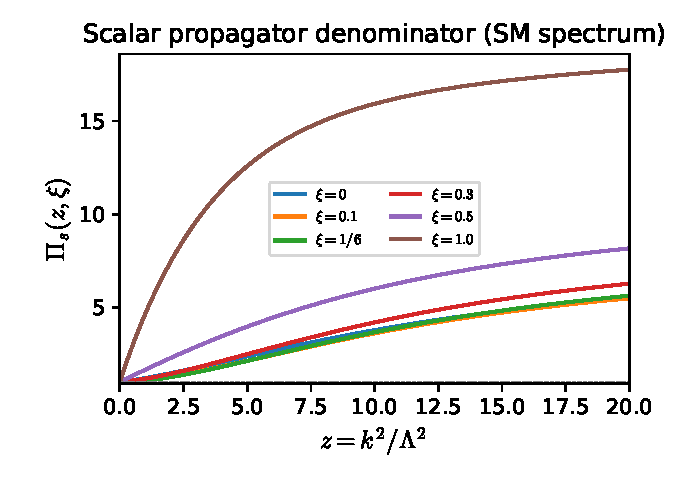
\includegraphics[width=0.85\columnwidth]{figures/fig1_pi_s_vs_z.pdf}
\caption{The scalar propagator denominator $\Pis(z,\xi)$ for six values
of the Higgs non-minimal coupling $\xi$. For all $\xi$, $\Pis > 1$
on the entire positive real axis: no scalar pole exists.
At $\xi = 1/6$ (conformal), $\Pis \equiv 1$.}
\label{fig:pi-s}
\end{figure}

\begin{figure}[t]
\centering
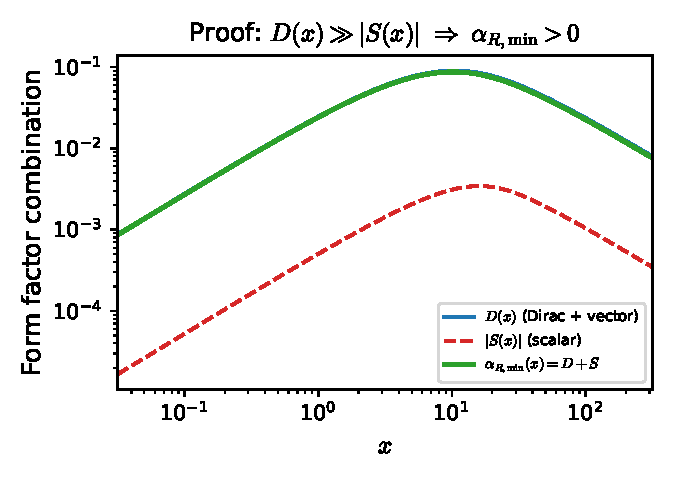
\includegraphics[width=0.85\columnwidth]{figures/fig2_D_vs_S.pdf}
\caption{Decomposition of $\alpha_{R,\min}(z) = D(z) + S(z)$
(Eq.~\ref{eq:alpha-min}). The Dirac+vector contribution $D(z)$
(blue) dominates the scalar contribution $|S(z)|$ (red dashed) by a
factor $> 20$ at all~$z$. The resulting $\alpha_{R,\min}$ (green)
is strictly positive.}
\label{fig:decomposition}
\end{figure}

\begin{figure}[t]
\centering
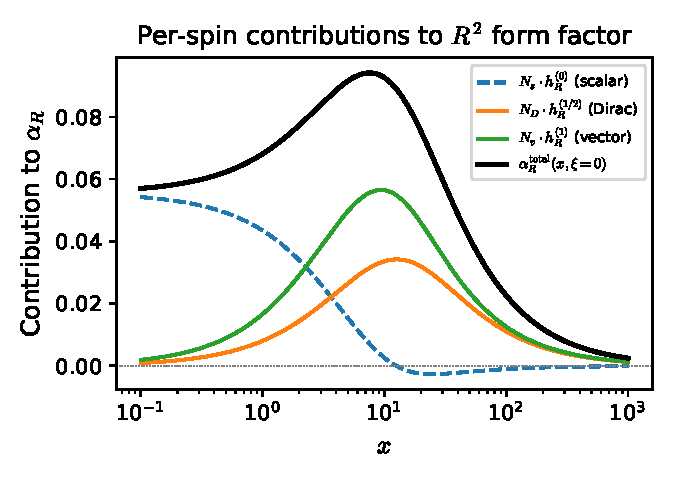
\includegraphics[width=0.85\columnwidth]{figures/fig5_per_spin_hR.pdf}
\caption{Per-spin contributions to the total $R^2$ form factor
$\alphaR(z,\xi\!=\!0)$. The scalar contribution (dashed) turns
negative for $z \gtrsim 15$, but the Dirac and vector contributions
(both always positive) ensure $\alphaR > 0$.}
\label{fig:per-spin}
\end{figure}

\begin{remark}
The physical mechanism is transparent: the conformal invariance of
massless Dirac fermions ($\beta_R^{(1/2)} = 0$) and gauge bosons
($\beta_R^{(1)} = 0$) in $d = 4$ means they contribute nothing to the
local $R^2$ coefficient but generate strictly positive nonlocal
$R^2$ corrections at $z > 0$. These corrections \emph{protect} the
scalar sector from developing a pole. The scalar fields alone (with
$N_f = N_v = 0$) \emph{do} produce a scalar graviton; it is the
conformal matter that eliminates it.
\end{remark}


% ======================================================================
\section{Degree-of-freedom count}
\label{sec:dof}
% ======================================================================

\begin{corollary}[SCT has exactly 2 gravitational DoF]
\label{cor:dof}
The physical gravitational spectrum of SCT consists of:
\begin{enumerate}[label=(\roman*)]
  \item the massless graviton (2 tensor polarizations, as in GR);
  \item the massive spin-2 mode at $m_2 = 1.554\,\Lam$, quantized
        as a fakeon (0 asymptotic DoF).
\end{enumerate}
No scalar gravitational mode exists. The no-scalaron result
(Theorem~\ref{thm:no-scalaron}) is independent of how the spin-2 mode
is quantized; the 2-DoF count additionally uses the Anselmi--Piva
fakeon prescription~\cite{Anselmi2017,AP2018}, which projects the
massive spin-2 state out of the asymptotic spectrum.

The fakeon propagator is the half-sum of retarded and advanced Green
functions, $G_f = (G_R + G_A)/2$. This is real (no absorptive part)
and Lorentz-invariant, but violates strict microcausality at distances
$r \lesssim 1/m_2$. Crucially, the violation is confined to the
Compton wavelength of the massive mode: for $\Lam \sim \mathrm{meV}$,
$1/m_2 \sim 100\,\mu$m, far below any macroscopic scale. The signal
front velocity remains exactly $c$ (the retarded propagator controls
the light cone), and the $S$-matrix remains unitary and Lorentz-covariant
order by order in perturbation theory~\cite{AP2018b}. Macroscopic
causality is therefore preserved; only the notion of a sharp microscopic
particle trajectory for the spin-2 mode is lost, which is consistent
with its absence from the asymptotic spectrum.
\end{corollary}

This should be contrasted with Stelle gravity~\cite{Stelle1977}
(8 helicity states: 2 massless + 5 massive spin-2 + 1 scalar),
$f(R)$ gravity (3~DoF, including a scalaron), and Ho\v{r}ava--Lifshitz
gravity (3~DoF, including an extra scalar).

In the Anselmi--Piva framework~\cite{AP2018b}, both the scalar and
spin-2 modes of generic quadratic gravity can be quantized as fakeons,
also yielding 2~physical DoF. The distinction is that in SCT the scalar
mode is \emph{absent at the propagator level} (no pole exists), rather
than being projected out by prescription. Furthermore, infinite-derivative
gravity (IDG)~\cite{BMS2012} achieves ghost-freedom by postulating an
entire-function form factor; in SCT, the form factors are \emph{derived}
from the spectral action with SM matter content.

The absence of the scalar mode eliminates the
van~Dam--Veltman--Zakharov (vDVZ) discontinuity~\cite{vDVZ1970,Zakharov1970}:
the SCT propagator smoothly reduces to the GR propagator as $\Lam \to \infty$,
with no extra $1/3$ contribution from a scalar exchange.


% ======================================================================
\section{Robustness under matter sector extensions}
\label{sec:robustness}
% ======================================================================

For a general matter spectrum with $N_s$ real scalars, $N_f$ Weyl
fermions, and $N_v$ gauge bosons, the no-scalaron condition
$\alpha_{R,\min}(z) > 0$ requires
\begin{equation}\label{eq:robustness}
  \frac{N_f}{2}\,h_R^{(1/2)}(z) + N_v\,h_R^{(1)}(z)
  > N_s\,|S_1(z)| \quad \text{for all } z > 0,
\end{equation}
where $S_1(z) = f_{R,\mathrm{bis}} - f_{RU}^2/(4f_U)$ is the
per-scalar contribution. The critical ratios are:
\begin{equation}\label{eq:critical}
  \frac{N_f}{N_s} > 2.37, \quad
  \frac{N_v}{N_s} > 0.25
  \quad \text{(either sufficient).}
\end{equation}
The SM values $N_f/N_s = 11.25$ and $N_v/N_s = 3.0$ exceed these
thresholds by factors of $4.7$ and $12$, respectively.

All physically motivated BSM extensions (sterile neutrinos, dark photon,
additional scalar singlet) preserve the no-scalaron theorem.
Only a \emph{pure scalar} theory ($N_f = N_v = 0$) develops a scalar
graviton, a scenario excluded by the observed matter content of the universe.
Figure~\ref{fig:robustness} shows the safe region in the
$(N_f/N_s,\; N_v/N_s)$ plane.

\begin{figure}[t]
\centering
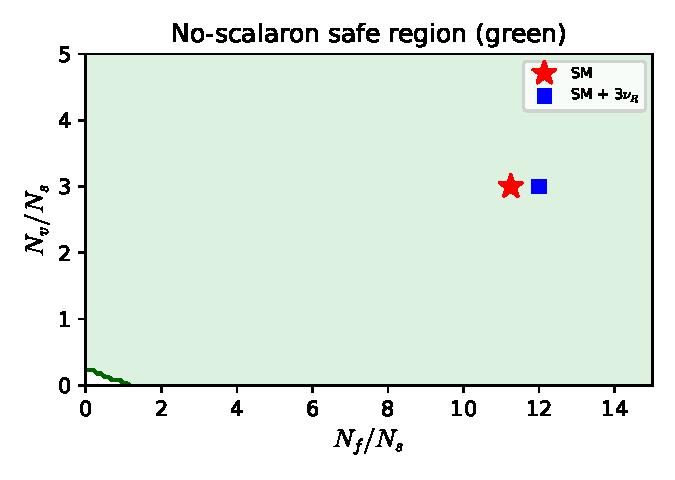
\includegraphics[width=0.85\columnwidth]{figures/fig3_robustness.pdf}
\caption{No-scalaron safe region (green) in the matter content plane
$(N_f/N_s,\; N_v/N_s)$. The SM (red star) lies deep inside the safe
region; BSM extensions (blue square: SM + 3 sterile neutrinos) remain
safe. The boundary is determined by the critical ratios~\eqref{eq:critical}.}
\label{fig:robustness}
\end{figure}


% ======================================================================
\section{Gravitational wave phenomenology}
\label{sec:gw}
% ======================================================================

\subsection{Speed and polarization}

On FLRW backgrounds, the Weyl tensor vanishes ($C_{\mu\nu\rho\sigma} = 0$),
and the tensor perturbation equation gives~\cite{Alfyorov2025b}
\begin{equation}
  c_T = c\;\bigl[1 + \mathcal{O}(H^2/\Lam^2)\bigr].
\end{equation}
For $\Lam \geq 3.53$~meV (torsion-balance bound, Eq.~\ref{eq:torsion}),
$|c_T/c - 1| \lesssim 10^{-62}$, trivially satisfying the
GW170817 constraint $|c_T/c - 1| < 5.6 \times 10^{-16}$~\cite{GW170817}.

The two tensor polarizations of GR are the only propagating modes.
No scalar breathing mode exists (Theorem~\ref{thm:no-scalaron}),
providing a falsifiable prediction for scalar polarization searches
in LIGO/Virgo/KAGRA and future detectors.


\subsection{Dispersion relation}

The linearized field equation $k^2\,\PiTT(k^2/\Lam^2)\,\tilde{h}_{\mu\nu} = 0$
factorizes into two branches:
\begin{equation}\label{eq:branches}
  k^2 = 0 \quad \text{(massless graviton)}, \qquad
  \PiTT(k^2/\Lam^2) = 0 \quad \text{(massive fakeon)}.
\end{equation}
The physical gravitational wave satisfies $\omega^2 = |\mathbf{k}|^2$
\emph{exactly} on flat backgrounds: the form factor modifies the wave
operator but does not shift the massless pole. The massive branch
$k^2 = z_0\Lam^2$ corresponds to the spin-2 fakeon (not an asymptotic
state).

On cosmological (FLRW) backgrounds, the Weyl tensor vanishes and the
tensor perturbation equation gives curvature-induced corrections
$\omega^2 = k^2[1 + \mathcal{O}(H^2/\Lam^2)]$, as proven by
explicit reduction of the full nonlocal field equations to FLRW
in Ref.~\cite{Alfyorov2025b} (Theorem~5.1 therein). For
$\Lam \gtrsim 1$~meV, this correction is $\lesssim 10^{-62}$ and
completely undetectable.

\begin{remark}
The coefficient $13/60$ in the Taylor expansion of $\PiTT$ appears in
the off-shell wave operator at $\mathcal{O}(k^4/\Lam^2)$ but does
\emph{not} modify the on-shell dispersion of the physical graviton.
A formal mapping to the Mirshekari--Yunes--Will
parametrization~\cite{MYW2012} gives $A_4^{\mathrm{formal}} = 13/(60\Lam^2)$,
which, using the GWTC-3 bound $A_4 < 3.0 \times 10^3~\mathrm{eV}^{-2}$~\cite{GWTC3},
yields $\Lam > 8.50$~meV. However, this is an off-shell constraint
on the wave operator coefficient, not a bound on physical GW
dispersion (which is identically zero in SCT on flat backgrounds).
\end{remark}


\subsection{Experimental bounds}

The strongest \emph{on-shell} constraint on $\Lam$ comes from the
dedicated torsion-balance analysis:
\begin{center}
\begin{tabular}{lrl}
\toprule
Channel & $\Lam_{\min}$ (meV) & Reference \\
\midrule
Torsion balance (Stelle approx.) & 2.38 & \cite{Alfyorov2025b} \\
\textbf{Torsion balance (SCT dedicated)} & \textbf{3.53} & this work, Eq.~\eqref{eq:torsion} \\
Off-shell MYW (GWTC-3, formal) & 8.50 & \cite{GWTC3} \\
\bottomrule
\end{tabular}
\end{center}
The dedicated torsion-balance bound ($3.53$~meV) is the strongest
on-shell constraint. The off-shell MYW bound ($8.50$~meV) from GWTC-3
constrains the wave operator coefficient but does not correspond to
physical GW dispersion (see Remark above).


% ======================================================================
\section{Discussion}
\label{sec:discussion}
% ======================================================================

\subsection{Comparison with other theories}

\begin{table}[H]
\centering
\caption{Gravitational spectrum of higher-derivative gravity theories.}
\label{tab:comparison}
\begin{tabular}{lcccl}
\toprule
Theory & Scalar & Spin-2 & DoF & UV behavior \\
\midrule
GR & --- & --- & 2 & non-renorm. \\
\textbf{SCT (this work)} & \textbf{no real pole} & \textbf{fakeon} & \textbf{2} & \textbf{one-loop} \\
Stelle (1977) & ghost & ghost & 8 & renorm. \\
$f(R)$ & scalaron & --- & 3 & non-renorm. \\
IDG & --- (postulated) & --- & 2 & finite (postulated) \\
Ho\v{r}ava--Lifshitz & extra mode & --- & 3 & power-counting \\
\bottomrule
\end{tabular}
\end{table}

SCT is distinguished from IDG by its \emph{derivation} from first
principles: the form factors arise from the spectral action with
SM matter content, not from a postulated entire function. The
no-scalaron theorem is a \emph{derived consequence}, not an input.

In Brans--Dicke theory~\cite{BransDicke}, the scalar mode decouples
only in the strong-coupling limit $\omega \to \infty$; in generic
scalar-tensor and Horndeski theories, the scalar is present for all
finite parameter values. In $f(R)$ gravity, a propagating scalaron
is an unavoidable consequence of the higher-derivative structure.
SCT is unique in that the scalar mode is eliminated by the
\emph{matter content} (conformal fermions and gauge bosons), not by
tuning a gravitational coupling to a special value.


\subsection{Perturbative stability}

The no-scalaron theorem is derived at one loop. At $L$ loops, the
form factors receive corrections proportional to $(G_N \Lam^2)^{L-1}$.
Since $G_N \Lam^2 = (\Lam/M_P)^2 \lesssim 10^{-60}$ for $\Lam$ at
the meV scale, higher-loop corrections to $\alphaR(z,\xi)$ are
suppressed by at least sixty orders of magnitude. Since the one-loop
value $\alphaR \sim 0.05$ is positive by a finite margin (not a
near-cancellation), a $10^{-60}$-level correction cannot change its
sign: no scalar pole can be generated perturbatively. The theorem is
therefore perturbatively stable. Non-perturbative effects
(gravitational instantons, infrared resummation) are beyond the
scope of the present one-loop analysis.


\subsection{Gravitational spectroscopy}

The results of this paper, combined with the fakeon
prescription~\cite{Anselmi2017}, yield the \emph{real-axis}
gravitational particle spectrum of SCT from the SM field content alone
(additional complex Lee--Wick poles exist; see the unitarity analysis):
\begin{center}
\begin{tabular}{lcl}
\toprule
Mode & Mass & Status \\
\midrule
Graviton & $0$ & 2 polarizations (as GR) \\
Spin-2 fakeon & $m_2 = 1.554\,\Lam$ & virtual only (0 asymptotic DoF) \\
Scalar & --- & absent (Theorem~\ref{thm:no-scalaron}) \\
\bottomrule
\end{tabular}
\end{center}
The entire spectrum is controlled by a single scale $\Lam$. If $\Lam$
is measured from any one channel (GW dispersion, short-range gravity,
or astrophysical observations), all other observables are
\emph{predicted} with no remaining freedom. This ``one-scale
spectroscopy'' is a direct consequence of the parameter-free nature
of the spectral action: the gravitational couplings $\alphaC$,
$\alphaR$, and the spin-2 mass ratio $m_2/\Lam$ are all fixed by
the SM particle content.


\subsection{Modified Newtonian potential}

The absence of the scalar mode simplifies the static gravitational
potential. In Stelle gravity~\cite{Stelle1977}, the Yukawa approximation
gives~\cite{Alfyorov2025b}
\begin{equation}\label{eq:V-stelle}
  \frac{V_{\mathrm{Stelle}}(r)}{V_N(r)}
  = 1 - \frac{4}{3}\,\ee^{-m_2 r} + \frac{1}{3}\,\ee^{-m_0 r},
\end{equation}
where $m_0 = \Lam\sqrt{6}$ is the scalar mass at $\xi = 0$.
The spin-2 and scalar Yukawa corrections cancel at $r = 0$, giving
$V_{\mathrm{Stelle}}(0) = 0$.

The no-scalaron theorem eliminates the scalar Yukawa
($\Pis$ has no zero), while the spin-2 contribution persists: the
static potential is insensitive to the fakeon prescription because
the retarded and advanced propagators coincide at zero
frequency~\cite{AP2018b}. Since $m_2$ depends only on $\alphaC$
(which is $\xi$-independent), the SCT potential for all $\xi$ reduces to
\begin{equation}\label{eq:V-sct}
  \boxed{\frac{V_{\mathrm{SCT}}(r)}{V_N(r)}
  = 1 - \frac{4}{3}\,\ee^{-m_2 r},}
\end{equation}
a single-Yukawa correction with $m_2 = 1.554\,\Lam$. This is simpler
than the Stelle potential~\eqref{eq:V-stelle} and qualitatively distinct:
\begin{itemize}
  \item $V_{\mathrm{SCT}}(0)/V_N = -1/3$ in the Yukawa approximation,
        vs.\ $V_{\mathrm{Stelle}}(0)/V_N = 0$ (exact cancellation);
  \item no attractive scalar tail at intermediate $r$;
  \item monotonic approach to $V_N$ from above for $r \gtrsim 1/m_2$
        (Fig.~\ref{fig:potential}).
\end{itemize}
We stress that both~\eqref{eq:V-stelle} and~\eqref{eq:V-sct} are
\emph{local} (Yukawa) approximations, valid for $r \gg 1/\Lam$. At
$r \lesssim 1/\Lam$, the full nonlocal form factors dominate and the
pointwise values $V(0)$ are not physical. In particular, the
$V_{\mathrm{Stelle}}(0) = 0$ cancellation is also an artifact of the
local approximation, not a genuine regularization of the Newtonian
singularity~\cite{Stelle1977}.

The absence of the scalar Yukawa has a clear physical consequence:
the partial cancellation between spin-2 and scalar corrections that
softens the potential at short distances in Stelle gravity does not
occur in SCT. Within the local approximation, the SCT potential
retains a $1/r$ singularity (with a repulsive sign). This means
that the no-scalaron theorem, while eliminating the scalar degree of
freedom, does \emph{not} by itself resolve the point-source
singularity. Short-distance regularization in SCT must come from a
different mechanism: the full nonlocal structure of the form factors
at $r \sim 1/\Lam$, or from a nonperturbative UV completion (which
is beyond the scope of the present one-loop analysis). This situation
is analogous to QED, where the one-loop vacuum polarization modifies
but does not remove the Coulomb singularity; the resolution requires
the full nonperturbative theory.

\begin{figure}[t]
\centering
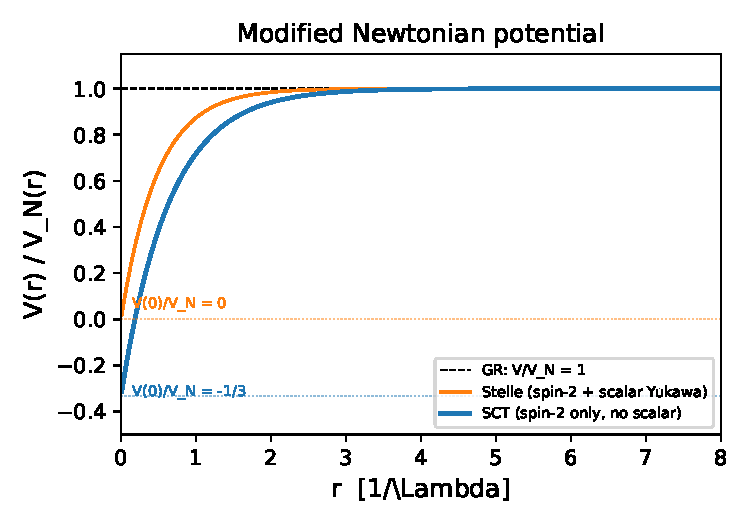
\includegraphics[width=0.85\columnwidth]{figures/fig6_potential.pdf}
\caption{Modified Newtonian potential $V(r)/V_N(r)$.
Stelle gravity (orange) has both spin-2 and scalar Yukawa corrections
that cancel at $r = 0$. SCT (blue) has only the spin-2 Yukawa
(Theorem~\ref{thm:no-scalaron} eliminates the scalar), producing a
repulsive core $V(0)/V_N = -1/3$.}
\label{fig:potential}
\end{figure}


\subsection{Falsifiability and experimental signatures}

The no-scalaron theorem leads to three distinct experimental signatures:

\paragraph{Scalar gravitational wave polarization.}
SCT predicts zero scalar breathing-mode amplitude for any $\xi$.
Detection of a scalar GW polarization in LIGO/Virgo/KAGRA or future
detectors (ET, CE) would rule out SCT. Current O3 bounds constrain
the scalar-to-tensor ratio to $\mathcal{O}(1)$; third-generation
detectors will reach $\mathcal{O}(10^{-2})$.

\paragraph{Dedicated torsion-balance bound.}
The SCT potential~\eqref{eq:V-sct} is a single-Yukawa correction with
amplitude $|\alpha| = 4/3$ and range $\lambda = 1/m_2 = 1/(1.554\,\Lam)$.
Using the Lee et~al.\ (2020)~\cite{Lee2020} exclusion curve at
$|\alpha| = 4/3$, the 95\% CL bound is $\lambda < 36.0\,\mu$m,
giving
\begin{equation}\label{eq:torsion}
  \Lam > \frac{\hbar c}{1.554 \times 36.0\,\mu\text{m}} = 3.53~\mathrm{meV}
  \quad \text{(torsion balance, dedicated).}
\end{equation}
This is $1.5\times$ stronger than the bound derived from the
double-Yukawa (Stelle) parametrization ($\Lam > 2.38$~meV) in
Ref.~\cite{Alfyorov2025b}, owing to the exact spin-2 mass
($m_2 = 1.554\,\Lam$ vs.\ $2.148\,\Lam$ locally) and the correct
signal amplitude ($|\alpha| = 4/3$, not rescaled from the
$|\alpha| = 1$ benchmark).

\emph{Caveat:} the Yukawa range $1/m_2 = 0.64/\Lam$ is comparable
to $1/\Lam$, the scale at which the full nonlocal propagator deviates
from the local approximation. The bound~\eqref{eq:torsion} should
therefore be regarded as an order-of-magnitude estimate; a precise
constraint requires the full nonlocal potential, which we defer to
future work.

\paragraph{Spectral action scale $\Lam$ from multiple channels.}
If $\Lam$ is measured from GW dispersion (GWTC-3 or future runs)
and independently from short-range gravity, the two values must
agree. The single parameter $\Lam$ controls both channels with no
freedom to adjust: inconsistency would falsify SCT.


% ======================================================================
\section{Conclusion}
\label{sec:conclusion}
% ======================================================================

We have proven that spectral causal theory propagates exactly two
gravitational degrees of freedom, the same as general relativity.
The scalar gravitational mode, which is generically present in
higher-derivative gravity, is universally absent due to the positive
contributions of conformal matter (fermions and gauge bosons) to the
$R^2$ form factor at nonzero momentum.

The key results are:
\begin{enumerate}
  \item \textbf{No-scalaron theorem} (Theorem~\ref{thm:no-scalaron}):
    $\alphaR(z,\xi) > 0$ and $\Pis(z,\xi) > 1$ for all $z > 0$ and
    all $\xi \in \mathbb{R}$, including conformal coupling. No real
    scalar mass pole exists. This is a parameter-free prediction from
    the SM spectrum.

  \item \textbf{Exact spin-2 mass:} $m_2 = 1.554\,\Lam$, a 38\%
    reduction from the local approximation ($m_2^{\mathrm{loc}} = 2.148\,\Lam$).

  \item \textbf{Torsion-balance bound:} $\Lam > 3.53$~meV (dedicated
    single-Yukawa analysis, $1.5\times$ stronger than the Stelle
    parametrization).

  \item \textbf{Robustness:} the SM lies $4.7\times$ (fermion) and
    $12\times$ (vector) above the critical thresholds; all BSM
    extensions preserve the theorem.

  \item \textbf{Falsifiability:} detection of scalar GW polarization
    at any frequency would rule out SCT.
\end{enumerate}

\bigskip
\noindent\textbf{Use of AI tools.}
Large language models (Claude, Anthropic) were used for code generation
and numerical verification scripting.
All mathematical derivations, physical arguments, and scientific conclusions
were formulated and verified by the authors. The AI-generated code was
independently validated against analytical results at 100-digit precision.

\bigskip
\noindent\textbf{Data availability.}
All numerical computations are reproducible from the publicly available
code repository~\cite{SCTrepo}.

\appendix
\section{Explicit form factor expressions}
\label{app:formulas}

All form factors are expressed in terms of the master function
$\varphi(z) = \int_0^1 \dd\alpha\;\ee^{-z\alpha(1-\alpha)}
= \ee^{-z/4}\sqrt{\pi/z}\;\mathrm{erfi}(\sqrt{z}/2)$,
with $\varphi(0) = 1$, $\varphi'(0) = -1/6$.

\paragraph{Dirac (spin-$\half$).}
\begin{equation}\label{eq:hR-dirac}
  h_R^{(1/2)}(z) = \frac{3\varphi + 2}{36\,z} + \frac{5(\varphi - 1)}{6\,z^2},
  \quad h_R^{(1/2)}(0) = 0.
\end{equation}

\paragraph{Vector (spin-1).}
\begin{equation}\label{eq:hR-vector}
  h_R^{(1)}(z) = -\frac{\varphi}{48} + \frac{11 - 6\varphi}{72\,z}
  + \frac{5(\varphi - 1)}{12\,z^2},
  \quad h_R^{(1)}(0) = 0.
\end{equation}

\paragraph{Scalar (spin-0).}
The scalar form factor decomposes as
$h_R^{(0)}(z,\xi) = f_{R,\mathrm{bis}}(z) + \xi\,f_{RU}(z) + \xi^2 f_U(z)$,
where
\begin{align}
  f_U(z) &= \varphi/2, \\
  f_{RU}(z) &= -\varphi/4 - (\varphi - 1)/(2z), \\
  f_{R,\mathrm{bis}}(z) &= \frac{1}{18\,z} + \frac{\varphi}{32}
    + \frac{\varphi}{8\,z} - \frac{7}{48\,z} - \frac{\varphi - 1}{8\,z^2}
    + \frac{\varphi - 1}{3\,z^2}.
\end{align}
The per-scalar contribution to the minimum is
$S_1(z) = f_{R,\mathrm{bis}} - f_{RU}^2/(4\,f_U)$, with UV asymptotics
$z\,S_1 \to -1/36$ and $z\,D \to 31/12$, giving
$|S/D|_{z\to\infty} = 4/93 \approx 0.043$.


\section{Derivation of the integral representations}
\label{app:integral-proofs}

Define moments $I_n(z) = \int_0^1 \tau^n \ee^{-z\tau}\,\dd\alpha$
with $\tau = \alpha(1-\alpha)$, so $I_0 = \varphi$.

Integration by parts using
$\tau'(\alpha) = 1-2\alpha$ and $(1-2\alpha)^2 = 1 - 4\tau$ yields
\begin{equation}\label{eq:L2}
  4z\,I_1 = (z+2)\,\varphi - 2,
\end{equation}
and for $n \geq 1$ the recurrence
\begin{equation}\label{eq:L1}
  4z\,I_{n+1} = (z + 4n + 2)\,I_n - n\,I_{n-1}.
\end{equation}

\paragraph{Proof of~\eqref{eq:g-integral}.}
From~\eqref{eq:L2} and~\eqref{eq:L1}, compute $I_2$ and $I_3$
explicitly.  Direct algebra then gives
$36z^2\,h_R^{(1/2)} = z^3(I_1 - 8I_2 + 16I_3)$.
Since $\tau - 8\tau^2 + 16\tau^3 = \tau(1-4\tau)^2 \geq 0$
(with $(1-4\tau) = (1-2\alpha)^2 \geq 0$),
the integrand is non-negative, establishing~\eqref{eq:g-integral}.

\paragraph{Proof of~\eqref{eq:h-integral}.}
Similarly, $144z^2\,h_R^{(1)} = 8z^3(I_1 - 5I_2 + 4I_3)$.
The kernel $\tau - 5\tau^2 + 4\tau^3 = \tau(1-\tau)(1-4\tau)$
is non-negative on $\tau \in [0, 1/4]$, establishing~\eqref{eq:h-integral}.


\section{Uniqueness of the spin-2 mass}
\label{app:uniqueness}

\begin{proposition}\label{prop:unique-zero}
$\PiTT(z)$ has exactly one positive real zero $z_0 \in (2, 5/2)$.
\end{proposition}

\begin{proof}[Proof sketch]
\emph{Step 1:} $\PiTT(z) > 0$ on $(0, 2]$.
Expand $\varphi$ to fourth order and bound $\PiTT$ below by a polynomial
$P_-(z) = 1 + \tfrac{13}{60}z - \tfrac{307}{840}z^2 + \tfrac{5}{112}z^3
- \tfrac{1}{140}z^4$, which is concave ($P_-'' < 0$ everywhere, since
discriminant $< 0$) and satisfies $P_-(0) = 1$, $P_-(2) = 3/14 > 0$.

\emph{Step 2:} $\PiTT(5/2) < 0$ from the upper Taylor bound.

\emph{Step 3:} At any positive zero $z_*$, expressing $\varphi(z_*)$ from
$\PiTT(z_*) = 0$ and using $4z\varphi' + (z+2)\varphi = 2$
(from~\eqref{eq:L2}) yields
\begin{equation}
  \PiTT'(z_*) = -\frac{996z_*^3 + 5799z_*^2 - 5600z_* - 8496}
  {24z_*(12z_*^2 + 93z_* + 236)}.
\end{equation}
For $z_* \geq 2$, the numerator factors as
$(z_*-2)(996z_*^2+7791z_*+9982) + 11468 > 0$,
so $\PiTT'(z_*) < 0$. A second zero would require $\PiTT$ to return
to zero from below, forcing $\PiTT'(z_2) \geq 0$, contradicting
$\PiTT'(z_2) < 0$.
\end{proof}


\begin{thebibliography}{99}

\bibitem{BV1985}
A.~O.~Barvinsky and G.~A.~Vilkovisky,
``The generalized Schwinger--DeWitt technique in gauge theories and
quantum gravity,''
Phys.\ Rep.\ \textbf{119}, 1 (1985).

\bibitem{CZ2012}
A.~Codello and O.~Zanusso,
``On the non-local heat kernel expansion,''
J.\ Math.\ Phys.\ \textbf{54}, 013513 (2013),
arXiv:1203.2034 [math-ph].

\bibitem{CC1996}
A.~H.~Chamseddine and A.~Connes,
``The spectral action principle,''
Commun.\ Math.\ Phys.\ \textbf{186}, 731 (1997).

\bibitem{CCM2007}
A.~H.~Chamseddine, A.~Connes, and M.~Marcolli,
``Gravity and the standard model with neutrino mixing,''
Adv.\ Theor.\ Math.\ Phys.\ \textbf{11}, 991 (2007).

\bibitem{Anselmi2017}
D.~Anselmi,
``On the quantum field theory of the gravitational interactions,''
JHEP \textbf{06}, 086 (2017).

\bibitem{AP2018}
D.~Anselmi and M.~Piva,
``The ultraviolet behavior of quantum gravity,''
JHEP \textbf{05}, 027 (2018).

\bibitem{Stelle1977}
K.~S.~Stelle,
``Renormalization of higher-derivative quantum gravity,''
Phys.\ Rev.\ D \textbf{16}, 953 (1977).

\bibitem{Sotiriou2010}
T.~P.~Sotiriou and V.~Faraoni,
``$f(R)$ theories of gravity,''
Rev.\ Mod.\ Phys.\ \textbf{82}, 451 (2010).

\bibitem{BMS2012}
T.~Biswas, E.~Gerwick, T.~Koivisto, and A.~Mazumdar,
``Towards singularity- and ghost-free theories of gravity,''
Phys.\ Rev.\ Lett.\ \textbf{108}, 031101 (2012).

\bibitem{AP2018b}
D.~Anselmi and M.~Piva,
``Quantum gravity, fakeons and microcausality,''
JHEP \textbf{11}, 021 (2018).

\bibitem{Alfyorov2025a}
D.~Alfyorov and I.~Shnyukov,
``Nonlocal one-loop form factors from the spectral action,''
Zenodo (2025), doi:10.22541/au.177507193.33027854/v1.

\bibitem{Alfyorov2025b}
D.~Alfyorov and I.~Shnyukov,
``Solar system and laboratory tests of spectral causal theory,''
Zenodo (2025), doi:10.22541/au.177524450.03515205/v1.

\bibitem{vDVZ1970}
H.~van~Dam and M.~J.~G.~Veltman,
``Massive and massless Yang--Mills and gravitational fields,''
Nucl.\ Phys.\ B \textbf{22}, 397 (1970).

\bibitem{Zakharov1970}
V.~I.~Zakharov,
``Linearized gravitation theory and the graviton mass,''
JETP Lett.\ \textbf{12}, 312 (1970).

\bibitem{GW170817}
B.~P.~Abbott \emph{et al.} [LIGO/Virgo],
``GW170817: Observation of gravitational waves from a binary neutron star
inspiral,''
Phys.\ Rev.\ Lett.\ \textbf{119}, 161101 (2017).

\bibitem{MYW2012}
S.~Mirshekari, N.~Yunes, and C.~M.~Will,
``Constraining Lorentz-violating, modified dispersion relations with
gravitational waves,''
Phys.\ Rev.\ D \textbf{85}, 024041 (2012).

\bibitem{GWTC3}
R.~Abbott \emph{et al.} [LIGO/Virgo/KAGRA],
``Tests of general relativity with GWTC-3,''
Phys.\ Rev.\ X \textbf{14}, 041017 (2024).

\bibitem{BransDicke}
C.~Brans and R.~H.~Dicke,
``Mach's principle and a relativistic theory of gravitation,''
Phys.\ Rev.\ \textbf{124}, 925 (1961).

\bibitem{Lee2020}
J.~G.~Lee, E.~G.~Adelberger, T.~S.~Cook, S.~M.~Fleischer, and B.~R.~Heckel,
``New test of the gravitational $1/r^2$ law at separations down to 52\,$\mu$m,''
Phys.\ Rev.\ Lett.\ \textbf{124}, 101101 (2020).

\bibitem{SCTrepo}
D.~Alfyorov,
``SCT Theory repository,''
Zenodo (2025), doi:10.5281/zenodo.19135673.

\end{thebibliography}

\end{document}
